\chapter{Noise}
\label{chap:noise}


\section{Noise distribution}

The electric noise in the readout stage is distributed according to a Gaussian distribution with zero mean and standard deviation $\sigma$, which is the quantity that charcterize the noise. During the readout, negative signal is clipped, so the observed noise distribution is the positive half of the starting distribution. This means that when we want to find $\sigma$, we have to take into account that the observed noise follows this new distribution.

\begin{figure}[h!]
    \centering
    \includegraphics[width=0.7\linewidth]{figures/noise/half_gaussian}
    \caption{Positive half Gaussian distribution. The mean of the distribution is $\mu_{pos} \simeq 0.8 \sigma$, and the standard deviation is $\sigma_{pos} \simeq 0.6 \sigma$. }
    \label{fig:half_gaussian}
\end{figure}
The mean and the standard deviation of the positive half of a Gaussian distribution centered in zero are

\begin{equation}
\mu_{pos} = \sigma \sqrt{\frac{2}{\pi}}, \quad \quad \sigma_{pos} = \sigma \sqrt{1 - \frac{2}{\pi}}.
\end{equation}

Given the distribution, we can find the maximum likelihood estimator for $\sigma^2$. The pdf of the distribution is the Gaussian distribution centered in zero and clipped below zero, thus it is

\begin{equation}
p(x; \sigma^2) = \frac{2}{\sqrt{2 \pi \sigma^2}} \exp{ \left( -\frac{x^2}{2\sigma^2} \right) }.
\end{equation}

The MLE estimator of $\sigma^2$, given $N$ measures for the single pixel can be calculated as

\begin{equation}
\frac{\partial \log \mathcal{L}(\sigma^2)}{\partial \sigma^2} = - \frac{N}{2\sigma^2} + \frac{\sum_i x_i^2}{2\sigma^4} = 0,
\end{equation}

which gives the estimator for $\sigma^2$.

\begin{equation}
\sigma^2_{MLE} = \frac{1}{N}\sum_ix_i^2.
\end{equation}

This estimator is unbiased and it is also guaranteed to be at the minimum variance bound, because the distribution belongs to the exponential family. Given that the Fisher information of the noise distribution is equal to the Gaussian's, the variance of $\sigma^2_{MLE}$ is

\begin{equation}
V(\sigma^2_{MLE}) = \frac{1}{NI} = \frac{2 \sigma^4}{N}.
\end{equation}

We want to know the standard deviation of the initial Gaussian distribution, so we have need to calculate the square root of the latter estimator. This new estimator is no more unbiased, but in the limit of a large sample, this property is recovered. Assuming to work with a large number of data for each pixel, we can also approximate the variance of $\sigma_{MLE}$ as

\begin{equation}
V(\sqrt{\sigma^2_{MLE}}) \simeq \left( \frac{\partial \sqrt{\sigma^2}}{\partial \sigma^2} \right)^2 V(\sigma^2_{MLE}) = \frac{\sigma^2}{2N}.
\end{equation}

Finally, the width of the noise Gaussian distribution for each pixel is

\begin{equation}
\hat{\sigma} = \sqrt{\frac{1}{N} \sum_i^N x_i^2} \pm \frac{\hat{\sigma}}{\sqrt{2N}}
\end{equation}


In practice, we find this value sampling the noise of each pixel for each event. The readout is performed with a padding of seven rows on top, and four rows and columns on the other directions. This means that the number of pixels read in an event is 130. To estimate the noise, it is necessary to remove the signal pixels. To do that, all the pixels around the seed pixels are removed from the noise analysis. Taking into account that the initial Gaussian distribution is symmetrical around zero, only half of the pixels have counts larger than zero, because there is no bias voltage. Thus the average number of pixels with a ADC larger than zero for each event is about 60. This number is essential to understand how many events we need to characterize the noise of each pixel within a certain relative error. Given that the relative error on $\hat{\sigma}$ is

\begin{equation}
\frac{\sigma_{\hat{\sigma}}}{\hat{\sigma}} = \frac{1}{\sqrt{2N}} \simeq \frac{0.707}{\sqrt{N}},
\end{equation}

if we want to achieve a certain relative error, we can calculate an estimate of the number of events that we need. The readout chip has $N_{pix} = 352\times 304$ pixels, and assuming that the signal events are uniformly distributed over the entire chip, the probability of a single pixel to be in the ROI is about $60 / N_{pix}$. The number of events to acquire is

\begin{equation}
N_{e} = \frac{N_{pix}}{60}N = \frac{N_{pix}}{60} \left( \frac{0.707}{\sigma_{\hat{\sigma}} / \hat{\sigma}} \right)^2.
\end{equation}

If we want a relative error of 3\% on $\sigma$, we need about $10^6$ events spread all across the readout chip. Pixels on the chip edges will have less statistics due to the ROI shape.


\begin{figure}[h!]
    \centering
    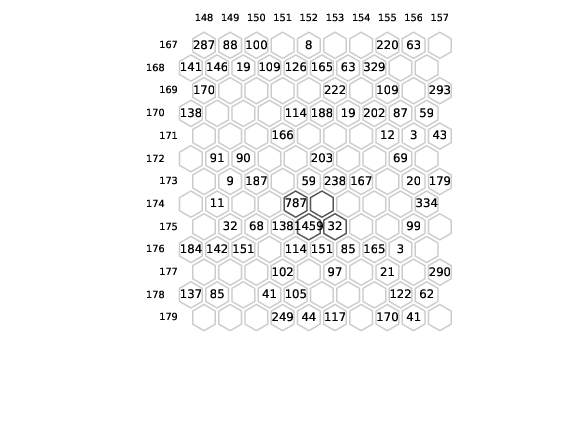
\includegraphics[width=0.7\linewidth]{figures/noise/noise_event}
    \caption{Example of readout for an event. Pixels with dark edges belong to the mini-cluster that activated the trigger, and defines the region-of-trigger (ROT). The totality of the pixels belong to the region-of-interest (ROI).}
    \label{fig:half_gaussian}
\end{figure}